 \documentclass[conference,a4paper]{IEEEtran}

\IEEEoverridecommandlockouts
% The preceding line is only needed to identify funding in the first footnote. If that is unneeded, please comment it out.
\usepackage{cite}   
\usepackage{amsmath,amssymb,amsfonts}
\usepackage{algorithmic}
\usepackage{graphicx}
\usepackage{textcomp}
\usepackage{subfig}
\usepackage{xcolor}
\usepackage{comment}
\usepackage{tikz}
\usetikzlibrary{positioning, arrows.meta, fit, backgrounds, calc, shapes.geometric, decorations.pathmorphing}
%\def\BibTeX{{\rm B\kern-.05em{\sc i\kern-.025em b}\kern-.08em
%    T\kern-.1667em\lower.7ex\hbox{E}\kern-.125emX}}



%% bare_conf.tex
%% V1.4b
%% 2015/08/26
%% by Michael Shell
%% See:
%% http://www.michaelshell.org/
%% for current contact information.
%%
%% This is a skeleton file demonstrating the use of IEEEtran.cls
%% (requires IEEEtran.cls version 1.8b or later) with an IEEE
%% conference paper.
%%
%% Support sites:
%% http://www.michaelshell.org/tex/ieeetran/
%% http://www.ctan.org/pkg/ieeetran
%% and
%% http://www.ieee.org/

%%*************************************************************************
%% Legal Notice:
%% This code is offered as-is without any warranty either expressed or
%% implied; without even the implied warranty of MERCHANTABILITY or
%% FITNESS FOR A PARTICULAR PURPOSE! 
%% User assumes all risk.
%% In no event shall the IEEE or any contributor to this code be liable for
%% any damages or losses, including, but not limited to, incidental,
%% consequential, or any other damages, resulting from the use or misuse
%% of any information contained here.
%%
%% All comments are the opinions of their respective authors and are not
%% necessarily endorsed by the IEEE.
%%
%% This work is distributed under the LaTeX Project Public License (LPPL)
%% ( http://www.latex-project.org/ ) version 1.3, and may be freely used,
%% distributed and modified. A copy of the LPPL, version 1.3, is included
%% in the base LaTeX documentation of all distributions of LaTeX released
%% 2003/12/01 or later.
%% Retain all contribution notices and credits.
%% ** Modified files should be clearly indicated as such, including  **
%% ** renaming them and changing author support contact information. **
%%*************************************************************************


% *** Authors should verify (and, if needed, correct) their LaTeX system  ***
% *** with the testflow diagnostic prior to trusting their LaTeX platform ***
% *** with production work. The IEEE's font choices and paper sizes can   ***
% *** trigger bugs that do not appear when using other class files.       ***                          ***
% The testflow support page is at:
% http://www.michaelshell.org/tex/testflow/

%\documentclass[conference]{IEEEtran}
% Some Computer Society conferences also require the compsoc mode option,
% but others use the standard conference format.
%
% If IEEEtran.cls has not been installed into the LaTeX system files,
% manually specify the path to it like:
% \documentclass[conference]{../sty/IEEEtran}





% Some very useful LaTeX packages include:
% (uncomment the ones you want to load)


% *** MISC UTILITY PACKAGES ***
%
%\usepackage{ifpdf}
% Heiko Oberdiek's ifpdf.sty is very useful if you need conditional
% compilation based on whether the output is pdf or dvi.
% usage:
% \ifpdf
%   % pdf code
% \else
%   % dvi code
% \fi
% The latest version of ifpdf.sty can be obtained from:
% http://www.ctan.org/pkg/ifpdf
% Also, note that IEEEtran.cls V1.7 and later provides a builtin
% \ifCLASSINFOpdf conditional that works the same way.
% When switching from latex to pdflatex and vice-versa, the compiler may
% have to be run twice to clear warning/error messages.






% *** CITATION PACKAGES ***
%
%\usepackage{cite}
% cite.sty was written by Donald Arseneau
% V1.6 and later of IEEEtran pre-defines the format of the cite.sty package
% \cite{} output to follow that of the IEEE. Loading the cite package will
% result in citation numbers being automatically sorted and properly
% "compressed/ranged". e.g., [1], [9], [2], [7], [5], [6] without using
% cite.sty will become [1], [2], [5]--[7], [9] using cite.sty. cite.sty's
% \cite will automatically add leading space, if needed. Use cite.sty's
% noadjust option (cite.sty V3.8 and later) if you want to turn this off
% such as if a citation ever needs to be enclosed in parenthesis.
% cite.sty is already installed on most LaTeX systems. Be sure and use
% version 5.0 (2009-03-20) and later if using hyperref.sty.
% The latest version can be obtained at:
% http://www.ctan.org/pkg/cite
% The documentation is contained in the cite.sty file itself.






% *** GRAPHICS RELATED PACKAGES ***
%
\ifCLASSINFOpdf
  % \usepackage[pdftex]{graphicx}
  % declare the path(s) where your graphic files are
  % \graphicspath{{../pdf/}{../jpeg/}}
  % and their extensions so you won't have to specify these with
  % every instance of \includegraphics
  % \DeclareGraphicsExtensions{.pdf,.jpeg,.png}
\else
  % or other class option (dvipsone, dvipdf, if not using dvips). graphicx
  % will default to the driver specified in the system graphics.cfg if no
  % driver is specified.
  % \usepackage[dvips]{graphicx}
  % declare the path(s) where your graphic files are
  % \graphicspath{{../eps/}}
  % and their extensions so you won't have to specify these with
  % every instance of \includegraphics
  % \DeclareGraphicsExtensions{.eps}
\fi
% graphicx was written by David Carlisle and Sebastian Rahtz. It is
% required if you want graphics, photos, etc. graphicx.sty is already
% installed on most LaTeX systems. The latest version and documentation
% can be obtained at: 
% http://www.ctan.org/pkg/graphicx
% Another good source of documentation is "Using Imported Graphics in
% LaTeX2e" by Keith Reckdahl which can be found at:
% http://www.ctan.org/pkg/epslatex
%
% latex, and pdflatex in dvi mode, support graphics in encapsulated
% postscript (.eps) format. pdflatex in pdf mode supports graphics
% in .pdf, .jpeg, .png and .mps (metapost) formats. Users should ensure
% that all non-photo figures use a vector format (.eps, .pdf, .mps) and
% not a bitmapped formats (.jpeg, .png). The IEEE frowns on bitmapped formats
% which can result in "jaggedy"/blurry rendering of lines and letters as
% well as large increases in file sizes.
%
% You can find documentation about the pdfTeX application at:
% http://www.tug.org/applications/pdftex





% *** MATH PACKAGES ***
%
%\usepackage{amsmath}
% A popular package from the American Mathematical Society that provides
% many useful and powerful commands for dealing with mathematics.
%
% Note that the amsmath package sets \interdisplaylinepenalty to 10000
% thus preventing page breaks from occurring within multiline equations. Use:
%\interdisplaylinepenalty=2500
% after loading amsmath to restore such page breaks as IEEEtran.cls normally
% does. amsmath.sty is already installed on most LaTeX systems. The latest
% version and documentation can be obtained at:
% http://www.ctan.org/pkg/amsmath





% *** SPECIALIZED LIST PACKAGES ***
%
%\usepackage{algorithmic}
% algorithmic.sty was written by Peter Williams and Rogerio Brito.
% This package provides an algorithmic environment fo describing algorithms.
% You can use the algorithmic environment in-text or within a figure
% environment to provide for a floating algorithm. Do NOT use the algorithm
% floating environment provided by algorithm.sty (by the same authors) or
% algorithm2e.sty (by Christophe Fiorio) as the IEEE does not use dedicated
% algorithm float types and packages that provide these will not provide
% correct IEEE style captions. The latest version and documentation of
% algorithmic.sty can be obtained at:
% http://www.ctan.org/pkg/algorithms
% Also of interest may be the (relatively newer and more customizable)
% algorithmicx.sty package by Szasz Janos:
% http://www.ctan.org/pkg/algorithmicx




% *** ALIGNMENT PACKAGES ***
%
%\usepackage{array}
% Frank Mittelbach's and David Carlisle's array.sty patches and improves
% the standard LaTeX2e array and tabular environments to provide better
% appearance and additional user controls. As the default LaTeX2e table
% generation code is lacking to the point of almost being broken with
% respect to the quality of the end results, all users are strongly
% advised to use an enhanced (at the very least that provided by array.sty)
% set of table tools. array.sty is already installed on most systems. The
% latest version and documentation can be obtained at:
% http://www.ctan.org/pkg/array


% IEEEtran contains the IEEEeqnarray family of commands that can be used to
% generate multiline equations as well as matrices, tables, etc., of high
% quality.




% *** SUBFIGURE PACKAGES ***
%\ifCLASSOPTIONcompsoc
%  \usepackage[caption=false,font=normalsize,labelfont=sf,textfont=sf]{subfig}
%\else
%  \usepackage[caption=false,font=footnotesize]{subfig}
%\fi
% subfig.sty, written by Steven Douglas Cochran, is the modern replacement
% for subfigure.sty, the latter of which is no longer maintained and is
% incompatible with some LaTeX packages including fixltx2e. However,
% subfig.sty requires and automatically loads Axel Sommerfeldt's caption.sty
% which will override IEEEtran.cls' handling of captions and this will result
% in non-IEEE style figure/table captions. To prevent this problem, be sure
% and invoke subfig.sty's "caption=false" package option (available since
% subfig.sty version 1.3, 2005/06/28) as this is will preserve IEEEtran.cls
% handling of captions.
% Note that the Computer Society format requires a larger sans serif font
% than the serif footnote size font used in traditional IEEE formatting
% and thus the need to invoke different subfig.sty package options depending
% on whether compsoc mode has been enabled.
%
% The latest version and documentation of subfig.sty can be obtained at:
% http://www.ctan.org/pkg/subfig




% *** FLOAT PACKAGES ***
%
%\usepackage{fixltx2e}
% fixltx2e, the successor to the earlier fix2col.sty, was written by
% Frank Mittelbach and David Carlisle. This package corrects a few problems
% in the LaTeX2e kernel, the most notable of which is that in current
% LaTeX2e releases, the ordering of single and double column floats is not
% guaranteed to be preserved. Thus, an unpatched LaTeX2e can allow a
% single column figure to be placed prior to an earlier double column
% figure.
% Be aware that LaTeX2e kernels dated 2015 and later have fixltx2e.sty's
% corrections already built into the system in which case a warning will
% be issued if an attempt is made to load fixltx2e.sty as it is no longer
% needed.
% The latest version and documentation can be found at:
% http://www.ctan.org/pkg/fixltx2e


%\usepackage{stfloats}
% stfloats.sty was written by Sigitas Tolusis. This package gives LaTeX2e
% the ability to do double column floats at the bottom of the page as well
% as the top. (e.g., "\begin{figure*}[!b]" is not normally possible in
% LaTeX2e). It also provides a command:
%\fnbelowfloat
% to enable the placement of footnotes below bottom floats (the standard
% LaTeX2e kernel puts them above bottom floats). This is an invasive package
% which rewrites many portions of the LaTeX2e float routines. It may not work
% with other packages that modify the LaTeX2e float routines. The latest
% version and documentation can be obtained at:
% http://www.ctan.org/pkg/stfloats
% Do not use the stfloats baselinefloat ability as the IEEE does not allow
% \baselineskip to stretch. Authors submitting work to the IEEE should note
% that the IEEE rarely uses double column equations and that authors should try
% to avoid such use. Do not be tempted to use the cuted.sty or midfloat.sty
% packages (also by Sigitas Tolusis) as the IEEE does not format its papers in
% such ways.
% Do not attempt to use stfloats with fixltx2e as they are incompatible.
% Instead, use Morten Hogholm'a dblfloatfix which combines the features
% of both fixltx2e and stfloats:
%
% \usepackage{dblfloatfix}
% The latest version can be found at:
% http://www.ctan.org/pkg/dblfloatfix




% *** PDF, URL AND HYPERLINK PACKAGES ***
%
%\usepackage{url}
% url.sty was written by Donald Arseneau. It provides better support for
% handling and breaking URLs. url.sty is already installed on most LaTeX
% systems. The latest version and documentation can be obtained at:
% http://www.ctan.org/pkg/url
% Basically, \url{my_url_here}.




% *** Do not adjust lengths that control margins, column widths, etc. ***
% *** Do not use packages that alter fonts (such as pslatex).         ***
% There should be no need to do such things with IEEEtran.cls V1.6 and later.
% (Unless specifically asked to do so by the journal or conference you plan
% to submit to, of course. )


% correct bad hyphenation here
\hyphenation{op-tical net-works semi-conduc-tor}


\begin{document}
%

\title{Our title }


% author names and affiliations
% use a multiple column layout for up to three different
% affiliations
\author{\IEEEauthorblockN{First Author and next author\\ and next author}
\IEEEauthorblockA{Science Club Spektrum, Poznan Univeristy of Technology\\
Polanka 3 Str, 60-965\\
Poznan, Poland\\
Email: krzysztof.cichon@put.poznan.pl}
%\and
%%\IEEEauthorblockN{Next author from another university}
%\IEEEauthorblockA{to be defined\\
%Email: }
%\and
%\IEEEauthorblockN{James Kirk\\ and Montgomery Scott}
%\IEEEauthorblockA{Starfleet Academy\\
%San Francisco, California 96678--2391\\
%Telephone: (800) 555--1212\\
%Fax: (888) 555--1212}
}

% make the title area
\maketitle

% As a general rule, do not put math, special symbols or citations
% in the abstract
\begin{abstract}
The abstract goes here.
\end{abstract}

% no keywords
\IEEEpeerreviewmaketitle



\section{Introduction}

The development of advanced wireless systems has increased interest in platforms based on software-defined radio (SDR), which enables flexible implementation of communication and sensing functions. By defining radio behavior primarily in software, SDR supports the evaluation of algorithms requiring programmable signal generation, adaptive signal processing chains, and runtime modification of system functionality during operation. This approach is relevant to distributed MIMO systems, adaptive beamforming, integrated sensing and communications (ISAC), and cooperative autonomous systems, where fixed hardware configurations impose significant limitations. \\
Conventional multi-antenna and multi-node experimental platforms are often limited by fixed geometries, limited scalability, and static node roles. Such limitations hinder the evaluation of algorithms that depend on spatial adaptation, dynamic configuration, or context-dependent operation, which are common in vehicular communications and distributed sensing scenarios. \\
To overcome these limitations, this work presents a mobile, modular, and centrally coordinated radio platform composed of multiple autonomous ground units operating as cooperative transmitters. Each unit integrates motion control, onboard computation, and an SDR frontend, enabling coordinated interaction between node positioning and radio operation. System coordination is performed by a centralized controller using a publish–subscribe communication model that maintains awareness of connected devices and synchronizes their operation.\\
The system architecture separates mobility control from radio processing and coordination. Motion is handled by embedded controllers, while waveform generation and algorithm execution are assigned to higher-performance computing units. This structure allows the same hardware platform to support multiple operational modes, including distributed beamforming, cooperative sensing, radio-based obstacle detection, and adaptive MIMO transmission, with mode changes performed at runtime.\\
The mobility of the radio nodes introduces an additional degree of freedom absent in conventional platforms. By actively controlling the spatial arrangement of transmitters and receivers, the system enables experimental investigation of directional energy focusing, environment-aware transmission, and spatial optimization strategies. Such capabilities are particularly relevant for studying scenarios where the propagation environment, target location, or interference conditions are not static. From an energy-efficiency perspective, spatial reconfiguration combined with adaptive signal processing allows the system to concentrate radiated power toward regions of interest, potentially reducing overall transmission energy while maintaining performance. \\
The proposed platform is designed as a general research framework rather than a solution tailored to a specific application. Its modular structure and algorithm-agnostic operation allow it to support a broad range of studies in wireless communication and sensing. The system can be applied to investigations related to autonomous vehicular systems, cooperative robotics, and distributed radar-like sensing.\\
In summary, the presented system enables the study of distributed and mobile wireless systems by combining programmable radio operation with controlled node mobility and centralized coordination. It provides a basis for investigating communication and sensing methods in dynamic and spatially adaptive scenarios.


\section{Mobile Unit Hardware Architecture}
\label{sec:unit_architecture}

Each mobile unit is built as a compact autonomous ground robot that integrates a drivetrain, embedded control electronics, an onboard computing platform, and a software-defined radio (SDR) front-end. The hardware architecture follows a layered design principle, in which each subsystem operates at a level of abstraction appropriate to its real-time requirements and computational complexity. Fig.~\ref{fig:unit_hw} presents a block diagram of a single mobile unit.

\begin{figure}[t]
\centering
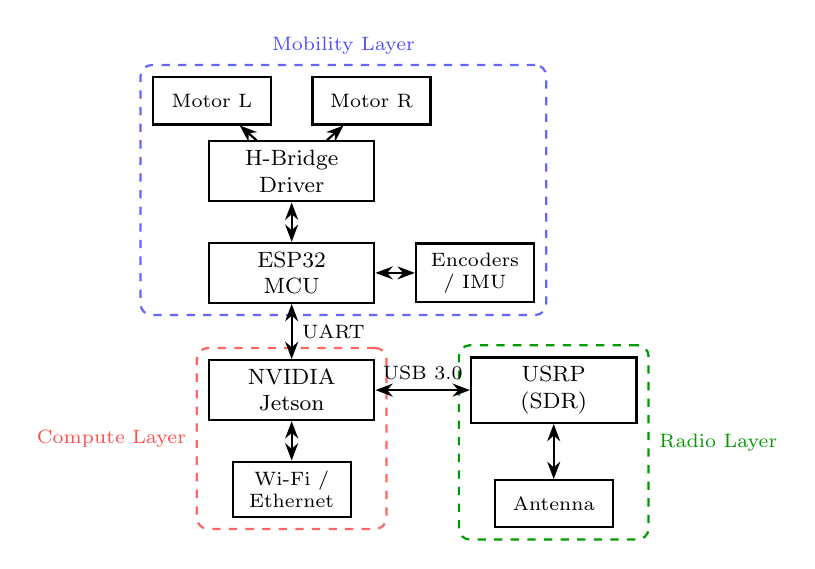
\begin{tikzpicture}[
    node distance=0.55cm and 0.8cm,
    block/.style={rectangle, draw, thick, minimum width=2.1cm, minimum height=0.75cm, align=center, font=\footnotesize},
    smallblock/.style={rectangle, draw, thick, minimum width=1.5cm, minimum height=0.6cm, align=center, font=\scriptsize},
    arr/.style={-{Stealth[length=2.2mm]}, thick},
    darr/.style={{Stealth[length=2.2mm]}-{Stealth[length=2.2mm]}, thick},
]
% --- Drive layer ---
\node[smallblock] (ml) {Motor L};
\node[smallblock, right=0.5cm of ml] (mr) {Motor R};
\node[block, below=0.5cm of $(ml)!0.5!(mr)$] (hbridge) {H-Bridge\\Driver};
\node[block, below=0.5cm of hbridge] (esp) {ESP32\\MCU};
\node[smallblock, right=0.5cm of esp] (enc) {Encoders\\/ IMU};

% --- Compute layer ---
\node[block, below=0.7cm of esp] (jetson) {NVIDIA\\Jetson};

% --- Radio layer ---
\node[block, right=1.2cm of jetson] (usrp) {USRP\\(SDR)};
\node[smallblock, below= 0.7cm of usrp] (ant) {Antenna};

% --- Network ---
\node[smallblock, below=0.5cm of jetson] (wifi) {Wi-Fi /\\Ethernet};

% --- Arrows ---
\draw[arr] (hbridge) -- (ml);
\draw[arr] (hbridge) -- (mr);
\draw[darr] (esp) -- (hbridge);
\draw[darr] (enc) -- (esp);
\draw[darr] (esp) -- node[right, font=\scriptsize]{UART} (jetson);
\draw[darr] (jetson) -- node[above, font=\scriptsize]{USB 3.0} (usrp);
\draw[darr] (usrp) -- (ant);
\draw[darr] (jetson) -- (wifi);

% --- Grouping ---
\begin{scope}[on background layer]
  \node[draw=blue!60, dashed, thick, rounded corners, fit=(ml)(mr)(hbridge)(esp)(enc), inner sep=4pt, label={[font=\scriptsize, blue!70]above:Mobility Layer}] {};
  \node[draw=red!60, dashed, thick, rounded corners, fit=(jetson)(wifi), inner sep=4pt, label={[font=\scriptsize, red!70]left:Compute Layer}] {};
  \node[draw=green!60!black, dashed, thick, rounded corners, fit=(usrp)(ant), inner sep=4pt, label={[font=\scriptsize, green!60!black]right:Radio Layer}] {};
\end{scope}
\end{tikzpicture}
\caption{Block diagram of a single mobile unit showing the three functional layers: mobility, compute, and radio.}
\label{fig:unit_hw}
\end{figure}

\subsection{Mobility Layer}
The drivetrain consists of two DC motors arranged in a differential-drive configuration, each connected to an H-bridge motor driver module. The H-bridge provides bidirectional control of motor current and allows pulse-width modulation (PWM)-based speed regulation. Both H-bridge channels are driven by an ESP32 microcontroller, which serves as the low-level mobility controller.

The ESP32 executes a real-time control loop that processes PWM commands, reads wheel encoder feedback, and acquires data from an onboard inertial measurement unit (IMU). These sensor inputs enable closed-loop velocity control and odometry estimation at the firmware level. Additionally, the ESP32 implements safety mechanisms including a software watchdog timer and emergency stop handling, ensuring that the mobility subsystem operates reliably and independently of higher-level software failures.

\subsection{Compute Layer}
The onboard computing platform is an NVIDIA Jetson module, which serves as the supervisory controller for the entire mobile unit. The Jetson communicates with the ESP32 via a wired serial interface (UART), through which it issues high-level motion commands (e.g., velocity setpoints, trajectory waypoints, turn commands) and receives telemetry data such as encoder counts, IMU readings, and battery status.

The separation between the ESP32 and the Jetson reflects a deliberate decomposition of real-time motor control (handled by the microcontroller) and computationally intensive tasks such as SDR signal processing (handled by the Jetson). This two-tier approach ensures deterministic motor control while enabling flexible, software-defined behavior at the application level.

\subsection{Radio Layer}
Each mobile unit carries a USRP software-defined radio connected to the Jetson via USB~3.0. The Jetson controls the USRP through the UHD (USRP Hardware Driver) framework, which provides programmatic access to transmission parameters, including carrier frequency, sampling rate, gain, and bandwidth. An omnidirectional antenna is mounted on the chassis to enable signal transmission.

In the current system configuration, the mobile units operate exclusively as transmitters. The Jetson hosts the transmit (TX) signal processing pipeline responsible for waveform generation and USRP control, while reception is handled by separate stationary receiver nodes (described in Section~\ref{sec:system_architecture}).


\section{System Architecture}
\label{sec:system_architecture}

The SignalTrack platform comprises three categories of nodes: four identical mobile transmitter units, two stationary receiver nodes, and a centralized system controller. All nodes are interconnected through a shared local area network. The overall system architecture is illustrated in Fig.~\ref{fig:system_arch}.

\begin{figure}[t]
\centering
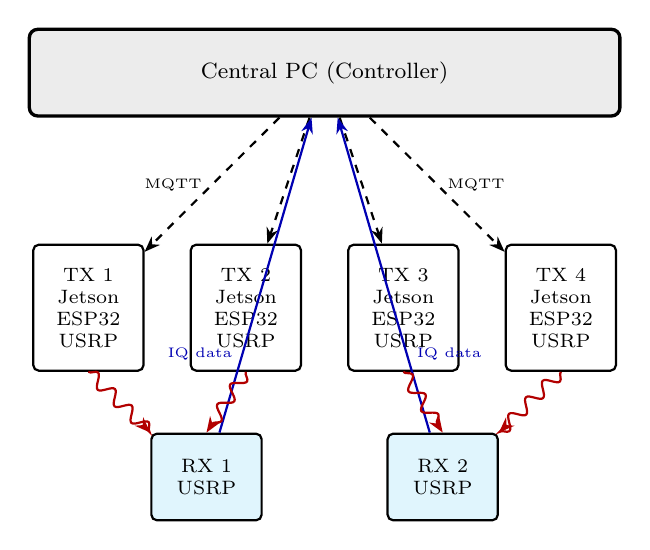
\begin{tikzpicture}[
    node distance=0.8cm and 0.6cm,
    unit/.style={rectangle, draw, thick, minimum width=1.4cm, minimum height=1.6cm, align=center, font=\scriptsize, rounded corners=2pt},
    rxnode/.style={rectangle, draw, thick, fill=cyan!12, minimum width=1.4cm, minimum height=1.1cm, align=center, font=\scriptsize, rounded corners=2pt},
    ctrl/.style={rectangle, draw, very thick, fill=gray!15, minimum width=7.5cm, minimum height=1.1cm, align=center, font=\footnotesize, rounded corners=3pt},
    arr/.style={-{Stealth[length=2mm]}, thick, dashed},
    darr/.style={{Stealth[length=2mm]}-{Stealth[length=2mm]}, thick, dashed},
    rf/.style={-{Stealth[length=2mm]}, thick, red!70!black, decorate, decoration={snake, amplitude=0.8mm, segment length=3mm}},
    iq/.style={-{Stealth[length=2mm]}, thick, blue!70!black},
]
% Central controller
\node[ctrl] (cc) {Central PC (Controller)};

% TX Units - evenly spaced row below controller
\node[unit, below=1.6cm of cc, xshift=-3.0cm] (u1) {TX 1\\\scriptsize Jetson\\\scriptsize ESP32\\\scriptsize USRP};
\node[unit, below=1.6cm of cc, xshift=-1.0cm] (u2) {TX 2\\\scriptsize Jetson\\\scriptsize ESP32\\\scriptsize USRP};
\node[unit, below=1.6cm of cc, xshift=1.0cm] (u3) {TX 3\\\scriptsize Jetson\\\scriptsize ESP32\\\scriptsize USRP};
\node[unit, below=1.6cm of cc, xshift=3.0cm] (u4) {TX 4\\\scriptsize Jetson\\\scriptsize ESP32\\\scriptsize USRP};

% RX Nodes
\node[rxnode, below=4.0cm of cc, xshift=-1.5cm] (rx1) {RX 1\\\scriptsize  USRP};
\node[rxnode, below=4.0cm of cc, xshift=1.5cm] (rx2) {RX 2\\\scriptsize  USRP};

% Control links (Central PC -> TX units)
\draw[arr] (cc) -- node[left, font=\tiny]{MQTT} (u1);
\draw[arr] (cc) -- (u2);
\draw[arr] (cc) -- (u3);
\draw[arr] (cc) -- node[right, font=\tiny]{MQTT} (u4);

% IQ links (RX -> Central PC)
\draw[iq] (rx1) -- node[left, font=\tiny, near start]{IQ data} (cc);
\draw[iq] (rx2) -- node[right, font=\tiny, near start]{IQ data} (cc);

% RF links (TX -> RX)
\draw[rf] (u1.south) -- (rx1.north west);
\draw[rf] (u2.south) -- (rx1.north);
\draw[rf] (u3.south) -- (rx2.north);
\draw[rf] (u4.south) -- (rx2.north east);

\end{tikzpicture}
\caption{System-level architecture of the SignalTrack platform. Four mobile transmitter units are controlled by a central PC via MQTT. Two stationary receiver nodes capture the transmitted RF signals and forward IQ~samples to the central PC for processing.}
\label{fig:system_arch}
\end{figure}

\subsection{Centralized Controller}
The system controller runs on a dedicated central PC connected to the same network as all other nodes. It fulfills two primary roles: (1)~orchestrating the mobile transmitter units, including issuing motion commands and configuring transmission parameters, and (2)~collecting and processing IQ~samples received from the stationary receiver nodes.

Communication between the central PC and the mobile units follows a publish--subscribe model based on the MQTT protocol. Each mobile unit, upon startup, registers its hardware capabilities (e.g., supported frequency bands, available TX channels) with the controller and reports readiness after successful initialization of the SDR hardware and onboard processing pipelines. During runtime, the controller publishes experiment parameters such as carrier frequency, waveform type, transmission schedule, per-unit phase or amplitude offsets, and mobility commands to the individual transmitter units.

The central PC also receives streamed IQ~samples from the two stationary receiver Jetsons over the network. These samples are used for centralized signal processing tasks, including beamforming weight computation, channel estimation, and performance evaluation.

\subsection{Stationary Receiver Nodes}
In addition to the four mobile transmitters, the system includes two stationary receiver nodes. Each receiver consists of an computer platform with a USRP front-end operating in receive mode. The receiver Jetsons capture IQ~samples from the over-the-air signals transmitted by the mobile units and forward these samples to the central PC for centralized processing.

The stationary placement of the receivers provides fixed and known reference positions, which simplifies calibration and beamforming weight calculation. The use of two spatially separated receivers also enables diversity reception and spatial analysis of the transmitted beam pattern.

\subsection{Distributed Beamforming Configuration}
In the initial operational mode, the system is configured for distributed transmit beamforming. The four USRP front-ends, each mounted on a separate mobile unit, operate as independent transmitters whose signals are intended to combine coherently at the receiver locations. The central PC applies a phase adjustment algorithm that iteratively modifies the per-unit transmission phase offsets based on the received signal quality reported by the stationary receivers.

\subsection{Scalability and Extensibility}
The modular design of both the mobile units and the communication infrastructure allows the system to scale beyond four transmitters or two receivers without architectural changes. Additional nodes can join the network by registering with the centralized controller. The MQTT-based communication model naturally supports dynamic addition and removal of nodes, making the platform suitable for experiments requiring variable array sizes or heterogeneous node configurations.


\section{Polaczenie systemu + samochodzik}
The integration of the central control system with the mobile units is realized through the reception and interpretation of control messages. The onboard computer acts as a gateway, directing specific commands to the appropriate subsystems based on the message content. This architecture ensures that instructions related to physical movement are routed to the embedded motion controller, while parameters concerning signal generation are directed to the software-defined radio frontend.

Message-based communication constitutes the primary system interface. The low-level mobility execution is handled by an embedded microcontroller (e.g., ESP32), which operates independently of the radio subsystem. This layer receives interpreted motion commands from the main message stream, ensuring that navigation tasks are executed reliably without burdening the high-level signal processing unit.

The core integration logic resides on the NVIDIA Jetson platform, which functions as the local computational node for both transmitter (TX) and receiver (RX) units. This platform hosts the software modules that interface with the USRP hardware via the UHD driver, translating high-level system commands into specific waveform configurations and transmission timings.

Although motion control and radio operations are handled by distinct hardware components, the message handling architecture unifies them into a coherent system. The communication framework ensures that a single control stream can efficiently synchronize vehicle positioning with radio transmission, maintaining a logical separation of duties while preserving system-wide consistency.

Connectivity with the centralized system controller is achieved through a publish–subscribe model based on the MQTT protocol. Upon startup, each mobile unit registers its capabilities and reports readiness only after the successful initialization of both the SDR hardware and the internal processing pipelines. During operation, the central controller issues experiment parameters, while the nodes return status updates or collected metrics.

The flexible nature of this message-based architecture supports various experimental scenarios, which may require different data exchange schemes. Depending on the specific algorithm loaded on the central controller, the message flow can be adapted—ranging from simple beacon transmission to complex, feedback-driven configurations—without requiring changes to the underlying vehicle firmware.

In summary, the architecture relies on a versatile message exchange protocol that enables a flexible binding between the central system logic and the distributed mobile hardware. This approach facilitates scalable coordination by abstracting the complexity of simultaneous motion and radio control into a unified communication interface.



\begin{figure}[!htbp]
    \centering
    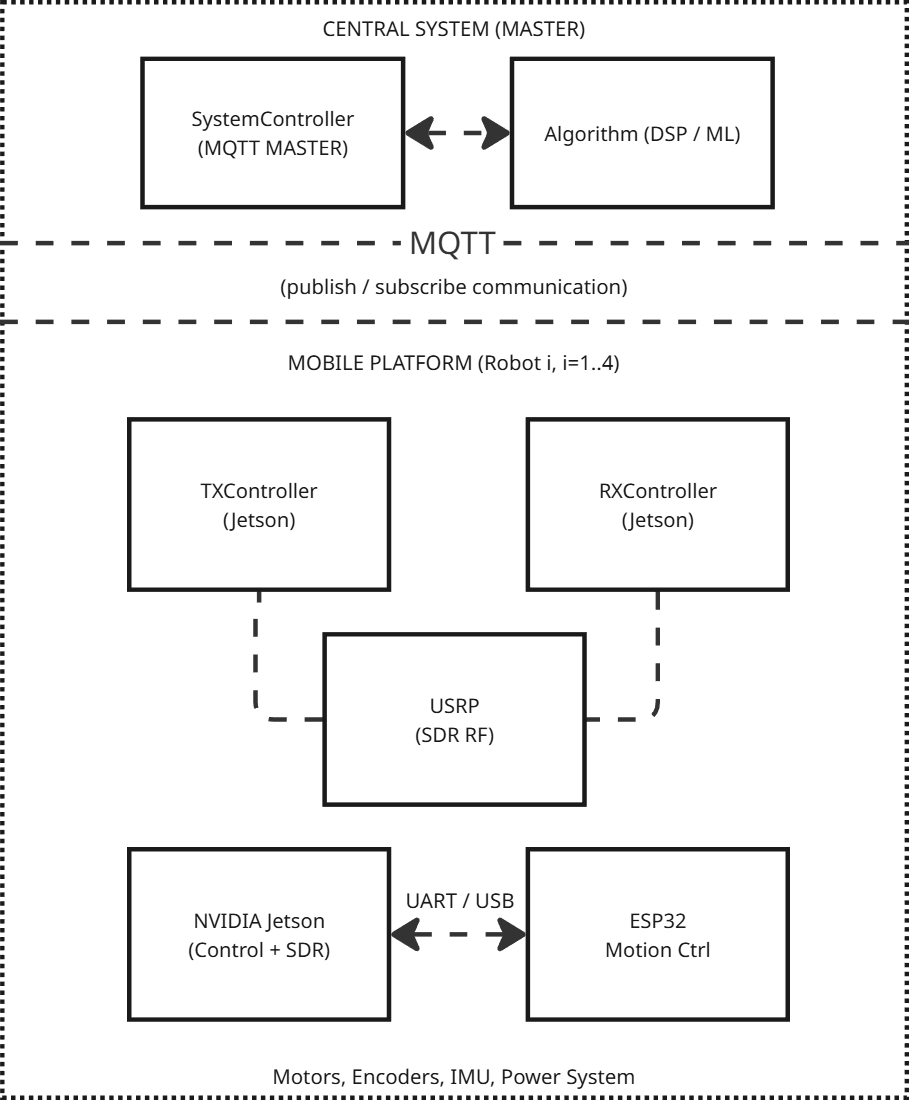
\includegraphics[width=\columnwidth{}]{central_system.png}
    \caption{System architecture of the SignalTrack platform integrating centralized SDR coordination with autonomous mobile units.}
    \label{fig:system_architecture}
\end{figure}



\section{Conclusion}
The conclusion goes here.
% conference papers do not normally have an appendix


% use section* for acknowledgment
\section*{Acknowledgment}

The authors would like to thank all the members of Science Club Spektrum involved in the work on the "Phantom6G" project.


% trigger a \newpage just before the given reference
% number - used to balance the columns on the last page
% adjust value as needed - may need to be readjusted if
% the document is modified later
%\IEEEtriggeratref{8}
% The "triggered" command can be changed if desired:
%\IEEEtriggercmd{\enlargethispage{-5in}}

% references section

% can use a bibliography generated by BibTeX as a .bbl file
% BibTeX documentation can be easily obtained at:
% http://mirror.ctan.org/biblio/bibtex/contrib/doc/
% The IEEEtran BibTeX style support page is at:
% http://www.michaelshell.org/tex/ieeetran/bibtex/
%\bibliographystyle{IEEEtran}
% argument is your BibTeX string definitions and bibliography database(s)
%\bibliography{IEEEabrv,../bib/paper}
%
% <OR> manually copy in the resultant .bbl file
% set second argument of \begin to the number of references
% (used to reserve space for the reference number labels box)
%\begin{thebibliography}{1}

%\bibitem{IEEEhowto:kopka}
%H.~Kopka and P.~W. Daly, \emph{A Guide to \LaTeX}, 3rd~ed.%\hskip 1em plus
%  0.5em minus 0.4em\relax Harlow, England: Addison-Wesley, 1999.

%\end{thebibliography}
\bibliographystyle{ieeetr}%{\raggedright\sloppy\small
\bibliography{bibliografia}
% that's all folks
\end{document}


